\documentclass[a4paper,10pt]{report}
\usepackage[utf8]{inputenc}
\usepackage{graphics}
\usepackage{graphicx}
% Title Page
\title{Eigenfaces vs. Fisherfaces: Recognition Using Class Specific Linear Projection}


\author{Khursheed ali (16305009 ),Ayush Goyal (16305R011)}
          
\begin{document}
\maketitle


\chapter{Methods}

\section{Correlation}
\textbf{attr database Accuracy:} 0.14 \\
\textbf{Yale database Accuracy:} 0.7 \\ 
Observation: Does't handle pose and illumination changes \\

\section{EigenFace}

\subsection{Experiments}
X-axis: Number of eigen Vectors(k)\\
Y-axis: Recognition rate
\newpage

\begin{enumerate}
 \item Attr Database
 \newline
 \textbf{Accuracy: 0.95 for k=29 }\\
 \begin{figure}[h]
	\centering
	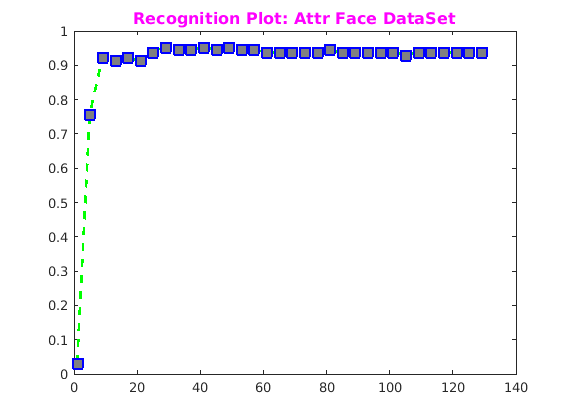
\includegraphics[scale=.6]{eigenattr.png}
	\caption{attr database}
	\label{fig.a}
\end{figure}


\newpage

\item Yale Database
 \newline
 \textbf{Accuracy: 0.39 for k=289 }\\

\begin{figure}[h]
	\centering
	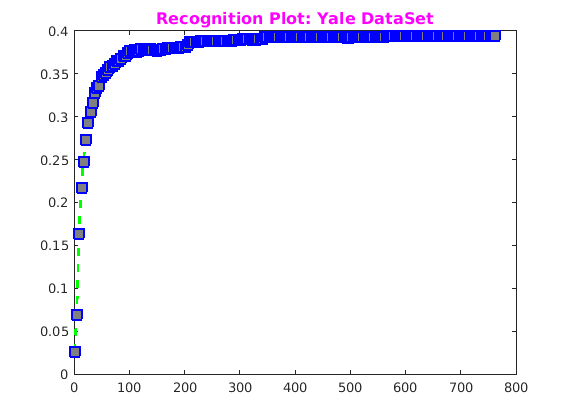
\includegraphics[scale=.6]{eigenYale.png}
	\caption{Yale database}
	\label{fig.b}
\end{figure}


\item Yale Database handling Illumination changes
 \newline
 \textbf{Accuracy: 0.68 for k=477 }\\

\begin{figure}[h]
	\centering
	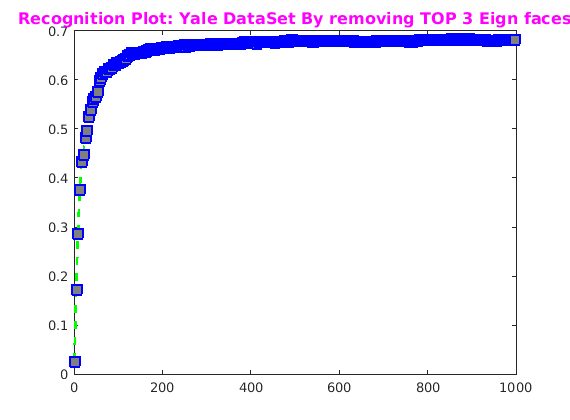
\includegraphics[scale=.6]{eigenYaleIllumination.png}
	\caption{Yale database handing illumination changes}
	\label{fig.c}
\end{figure}
\end{enumerate}
\newpage

\section{Fisher Face}

\textbf{ Function for Fisher Face :} \\
$W_{opt}$ = $argmax_W  \mid W_T S_B W \mid / \mid W_T S_W W \mid $\\
where $W_{opt}$ is optimal projection \\
      $S_B$ is between class scatter \\
      $S_W$ is within class scater \\

\newline

\noindent
\textbf{Problem}: To obtain the Fisherfaces, we need to compute the inverse of $S_w$ , i.e., $S_w^{-1}$ . 
If the sample feature vectors are defined in a p-dimensional space and p is larger than the total number of samples n , then $S_w$ is singular. \\
\textbf{Solutions}: There are three typically used solutions to this problem.
\begin{enumerate}
 \item In the first solution, we project the sample vectors onto the PCA space of r dimensions, with r$<=$rank($S_w$) and compute 
 the Fisherfaces in this PCA space.
 \item The second solution is to project the between- and within-class scatter matrices onto the PCA space of r dimensions, with r$<=$rank($S_w$) and compute 
 the Fisherfaces in this PCA space.
 
 
 \item The third solution is to add a regularising term to $S_w$.
That is, $S_w+\epsilon I$ , where I is the identity matrix and $\epsilon$ is a small constant.
\end{enumerate}

\textbf{We have tested for both Second and third Method.} Both methods give almost same results.\\

\subsection{Optimization used for second method}
\textbf{Problem:} Size of image vector was i.e d=H*W(32256 $\times$ 1 for Yale database). So Size of $S_B$ and $S_W$(scatter matix) was d $\times$ d(i.e 32256 $\times$ 32256), 
which is equal to 7.8 gb each. Finding $S_W$ and $S_B$ was a computation and memory overhead. \\
\textbf{Optimization:} To reduce computation and memory overhead we have used following method.\\
\begin{enumerate}
 \item For finding projected value of $S_B$ :\\ \\
 Mean vector for a particular class of Image=$\mu_i$\\ \\
 Mean Image vector all class images= $\overline{\mu}$\\ \\
 $\overline{\mu_i}$=$\mu_i-\overline{\mu}$\\ \\
 A=$[\hspace{0.1cm} \overline{\mu_1}*\sqrt{n_1}$  \hspace{0.2cm}   $\overline{\mu_2}*\sqrt{n_2} $ \hspace{0.2cm}... $ ] $\\ \\ 
 $S_B = AA^T$\\ \\ 
 $W_{PCA}^T S_B W_{PCA}= W_{PCA}^T.A.A^T.W_{PCA} $\\ \\
 $W_{PCA}^T S_B W_{PCA}= (W_{PCA}^T.A).(A^T.W_{PCA}) $ \\ \\
 Dimension of $W_{PCA}^T.A=(N-c) \times (N) $ ,where N in number of images and c in number of class \\ 
 
 \item For finding projected value of $S_W$ \\ \\
 Image vector of a class=$X_i$\\ \\
 Mean Image vector of a particular class = $\overline{\mu_{ci}}$\\ \\
 $\overline{X_i}$=$X_i-\overline{\mu_{ci}}$\\ \\
 B=$[\hspace{0.1cm} \overline{X_1}$  \hspace{0.2cm}   $\overline{X_2}$ \hspace{0.2cm}... $ ] $\\ \\ 
 $S_W = BB^T$\\ \\ 
 $W_{PCA}^T S_W W_{PCA}= W_{PCA}^T.B.B^T.W_{PCA} $\\ \\
 $W_{PCA}^T S_W W_{PCA}= (W_{PCA}^T.B).(B^T.W_{PCA}) $ \\ \\
 Dimension of $W_{PCA}^T.B=(N-c) \times (N) $ ,where N in number of images and c in number of class \\ 
 
 
\end{enumerate}






\subsection{Experiments}
\begin{enumerate}
 \item Attr Database
 \newline
 \textbf{Accuracy: 0.906250}\\
 \begin{figure}[h]
	\centering
	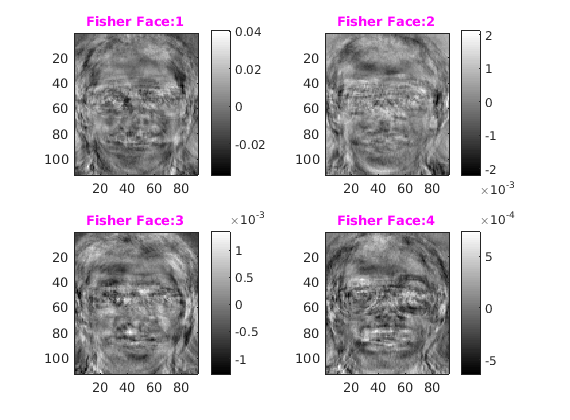
\includegraphics[scale=.6]{attrFisher.png}
	\caption{Fisher Faces for Attr Databse}
	\label{fig.d}
\end{figure}
\newpage
 \item Yale Database
 \newline
 \textbf{Scaling: 1}
  \newline
 \textbf{Accuracy: 0.739474 }\\
  \begin{figure}[h]
	\centering
	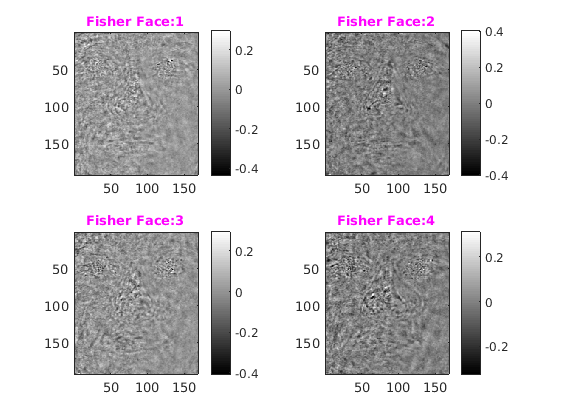
\includegraphics[scale=.6]{yaleScale1.png}
	\caption{Fisher Faces for Yale Databse}
	\label{fig.d}
\end{figure}

 \item Yale Database 
 \newline
 \textbf{Scaling: 0.5}
  \newline
 \textbf{Accuracy: 0.781579 }\\
  \begin{figure}[h]
	\centering
	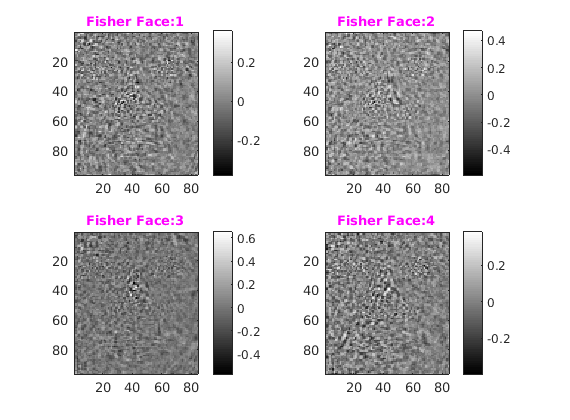
\includegraphics[scale=.6]{yaleScaleHalf.png}
	\caption{Fisher Faces for Yale Databse}
	\label{fig.e}
\end{figure}

\newpage

  \item Extended Yale Database
  \newline
   \textbf{Accuracy: 0.93 }\\
  \begin{figure}[h]
	\centering
	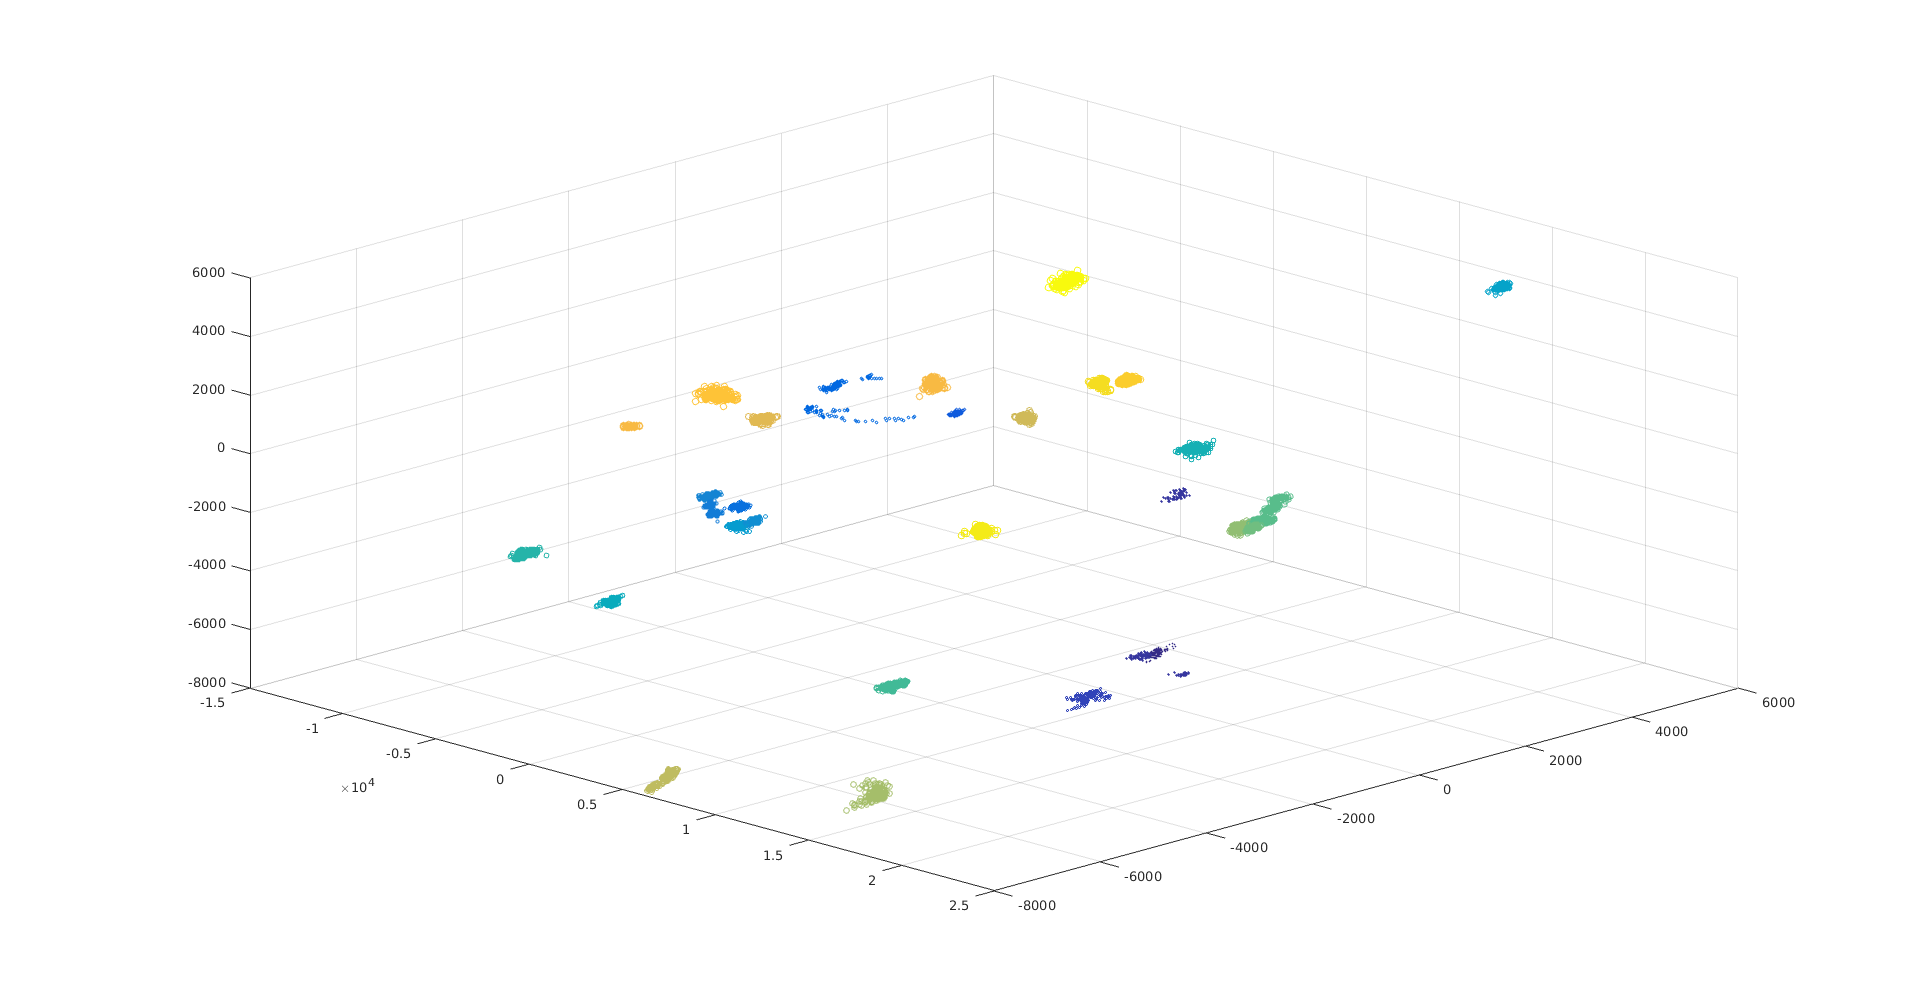
\includegraphics[scale=.35]{extendedYale.png}
	\caption{projection of test images on first 3 Fisher Face Vectors }
	\label{fig.f}
\end{figure}
\end{enumerate}






\end{document}          





